\section{Introduction}
\label{sec:intro}
Programming systems that interact with physical processes are gaining importance for robotics, manufacturing, IoT, and other cyber-physical systems. Traditional domain specific languages and models for these systems are platform specific as they combine various low-level sensing, communication, and control tasks with the higher-level applications~\cite{nordmann2014robotics}. For sophisticated high-level software applications, the tight-coupling of application design with platform-specific details hinders development, portability, code reuse,  verification, and synthesis.

This need for raising the level of abstraction and separating the \emph{platform-independent} decision and coordination tasks from \emph{platform-dependent} concerns such as sensing, communication, and low-level control motivates our work. For example, to develop an application for distributed package delivery with mobile robots in a building, the code for assigning robots to visit way-points in different rooms, load-balancing, and handling failures.  This application design is independent of the underlying platform, and therefore, should ideally be transferable across platforms. In contrast, steering control of the individual vehicles, indoor positioning, and message-level communication protocols are tied to the specific hardware.

%


Contrast that with the development of a similar location-based application for a heterogeneous collection of mobile robots. 
There are no languages for programming  robots that give the programmer the high-level of abstractions to say, for example, ``move from $A$ to $B$ avoiding $U$''. 
ROS~\cite{ros} provides many useful packages that work across different platforms, but it does not provide needed programming abstractions nor the compiler support. 
There is also a paucity of tools for deploying the generated code on the actual robots. 
Integrated, testing and validation tools for distributed robotic systems are also currently not available. 
Consequently, developing and debugging the application, even based on textbook algorithms, will take weeks. 
Since heterogeneous robotic platforms can be used for many tasks like mapping, surveillance, delivery, coordination,  the absence of the development ecosystem means that each application has to be developed from scratch with little reuse, modularity, or portability. 


In this paper, we address this gap by introducing {\em CyPhyHouse}\footnote{\href{https://cyphyhouse.github.io/index.html}{https://cyphyhouse.github.io}}: an open source software framework for programming, rapid deployment, and testing of distributed robotics applications. 
\sayan{The high-level $\lgname$ language enables users to write succinct distributed coordination applications without getting bogged down by messaging and thread management issues (See Examples in \reffig{lineform} and \reffig{taskapp}).}
Using the CyPhyHouse framework around $\lgname$, a user can code, compile, launch, and run applications in a highly-automated fashion (\reffig{arch}). 
\sayan{The framework has been built over three years and has more than 100k lines of source code.}
%
%\begin{figure}[h!]
%\centering
%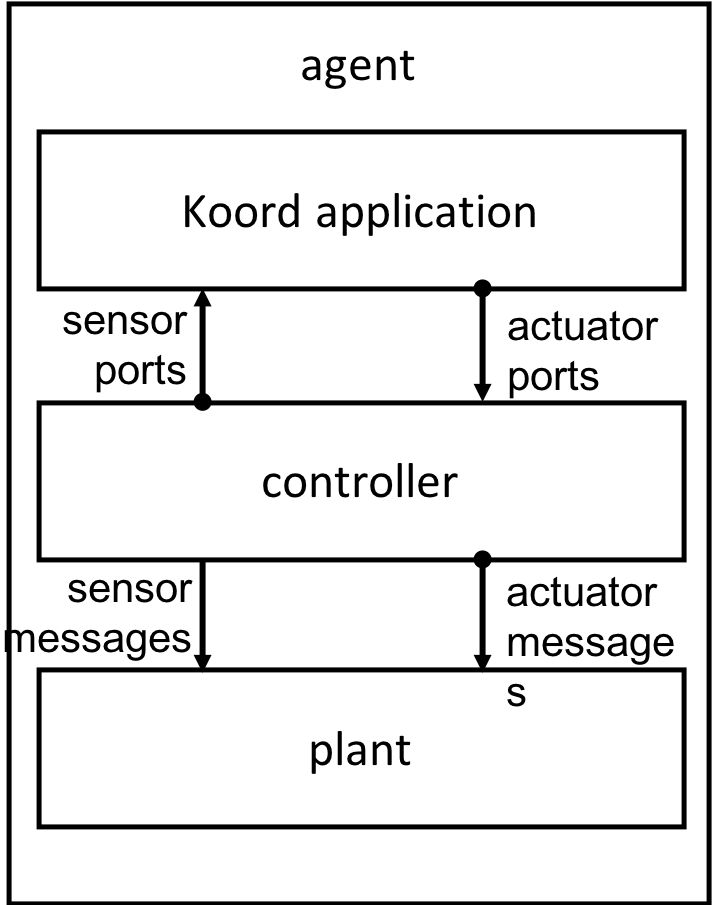
\includegraphics[width=0.48\textwidth]{figs/arch.png}
%\caption{\small CyPhyHouse framework. Major tools shown in blue.}
%\label{fig:arch}
%\end{figure}
%
The technical contributions of this paper are:
\begin{itemize}
\item Design and development of the CyPhyHouse open source software system. This includes a discrete event simulator for distributed robotic systems, the application launcher, the run-time logging and monitoring system, and an integrated indoor positioning system. All of these software tools are integrated with our new robot programming language called $\lgname$ and its compiler. 
\item First demonstration of the feasibility of end-to-end high-level application development and deployment on a distributed, heterogeneous, platform involving quadcopters and ground vehicles. 
\item Demonstration of the feasibility of system-level verification of applications written in $\lgname$. 
\end{itemize}
Design and development of the $\lgname$ programming language and the supporting $\mathbb{K}$-based~\cite{Kpaper} verification tool \kbmc\, are discussed here for the sake of completeness; those details will appear elsewhere~\cite{koordreport}.

%Design and development of the Koord programming language and the supporting verification tool KoordBMC~\cite{koordreport}--- significant, related but separate efforts---are not contributions of the current paper; we discuss their usage for the sake of completeness. 
% completely describing the framework. 
% the Demonstration of an example application development using CyPhyHouse tools and deployment on a physical system using multiple quadcopters.
%Non-contributions: Spell these out  to avoid misdirected criticisms and conflict with overlapping publications.
%\begin{itemize} 
%\item Language design
%\item Verification tools.
%\item Low-level controller design for vehicles.
%\end{itemize} 

%\begin{figure}[h!]
%\centering
%\includegraphics[width=0.45\textwidth]{figs/exp_traces.png}
%\caption{\small Experimental run in our testbed. The traces show the path of each robot for the last $2$ seconds. }
%\label{fig:exp_traces}
%\end{figure}



    - problems in the space of (distributed) CPS, robotics, automation .
    - Coordination and Control issues. 
    - why we need something like Koord /why something like koord helps computer scientists (non roboticists) work with robotics. 
    - what is koord and how Koord specifically accommodates users
    - how we built koord. 
    - what is this paper
    - Related work
